% id: 0323
% book: RPM 기하 · 03 공간도형
% section: 유형 UP 14 정사영의 넓이의 실생활에서의 활용
% figure: crop:fig-0323.png
% answer: ②
% answer_source: 답지(쪽 렌더)
% variant_level: 0 (원본 전사)
% 이 파일은 build.mjs 가 items.json 에서 만든다. 고칠 때는 items.json 을 고친다.
\smash{\raisebox{1.5mm}{\dmkichul{RPM 기하 0323번 · 52쪽 · 대표문제}}}
\noindent\begin{minipage}[t]{0.58\linewidth}\vspace{0pt}\raggedright 오른쪽 그림과 같이 반지름의 길이가 $5\mkern3mu \mathrm{m}$인 구 모양의 애드벌룬이 지면 위에 떠 있다. 태양 광선이 지면과 $30^\circ$의 각을 이루면서 비출 때, 지면 위에 생긴 애드벌룬의 그림자의 넓이는?\end{minipage}\hfill\begin{minipage}[t]{0.4\linewidth}\vspace{0pt}\centering \setlength{\dmfigw}{111.6pt}\ifdim\dmfigw>\linewidth\setlength{\dmfigw}{\linewidth}\fi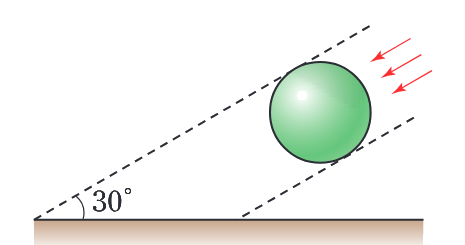
\includegraphics[width=\dmfigw]{figures/fig-0323.png}\end{minipage}\par
\begin{choices32}{\rule[-3ex]{0pt}{8ex}$45\pi\mkern3mu \mathrm{m}^2$}{\rule[-3ex]{0pt}{8ex}$50\pi\mkern3mu \mathrm{m}^2$}{\rule[-3ex]{0pt}{8ex}$40\sqrt{3}\pi\mkern3mu \mathrm{m}^2$}{\rule[-3ex]{0pt}{8ex}$70\pi\mkern3mu \mathrm{m}^2$}{\rule[-3ex]{0pt}{8ex}$50\sqrt{3}\pi\mkern3mu \mathrm{m}^2$}\end{choices32}
